% Raport techniczny: system wspomagania decyzji dla inspekcji sanitarnej w Chicago.
% Dane i liczby:  uv run python docs/tech-report/export_data.py   (po `insp train` i `insp evaluate`)
% Kompilacja:     pdflatex report.tex && pdflatex report.tex
\documentclass[11pt,a4paper]{article}

\usepackage[utf8]{inputenc}
\usepackage[T1]{fontenc}
\usepackage[polish]{babel}
\usepackage{lmodern}
\usepackage{microtype}
\usepackage[a4paper,margin=2.5cm]{geometry}
\usepackage{parskip}
\usepackage{graphicx}
\usepackage{amsmath}
\usepackage{array}
\usepackage{booktabs}
\usepackage{tabularx}
\usepackage{enumitem}
\usepackage[font=small,labelfont=bf]{caption}
\usepackage{subcaption}
\usepackage{xcolor}
\usepackage{tikz}
\usetikzlibrary{arrows.meta,positioning}
\usepackage{pgfplots}
\usepackage{pgfplotstable}
\usepgfplotslibrary{groupplots}
\pgfplotsset{compat=1.18}
\usepackage{hyperref}

% Generated by export_data.py; do not edit by hand.
\newcommand{\NInspections}{316\,636}
\newcommand{\NPlaces}{49\,270}
\newcommand{\FirstYear}{2010}
\newcommand{\DataUntil}{21.10.2026}
\newcommand{\MandatoryShare}{46}
\newcommand{\MedianDaily}{76}
\newcommand{\RoutinePerDay}{35}
\newcommand{\RefDay}{20.10.2026}
\newcommand{\DueRef}{7\,481}
\newcommand{\NTrain}{70\,027}
\newcommand{\NValid}{8\,571}
\newcommand{\NTest}{13\,447}
\newcommand{\AucValidGB}{0,638}
\newcommand{\BrierValidGB}{0,171}
\newcommand{\TopValidGB}{42,0}
\newcommand{\AucTestGB}{0,626}
\newcommand{\BrierTestGB}{0,168}
\newcommand{\TopTestGB}{35,0}
\newcommand{\AucValidLR}{0,629}
\newcommand{\BrierValidLR}{0,172}
\newcommand{\TopValidLR}{40,8}
\newcommand{\AucTestLR}{0,626}
\newcommand{\BrierTestLR}{0,169}
\newcommand{\TopTestLR}{36,6}
\newcommand{\AllValid}{23,2}
\newcommand{\AllTest}{22,3}
\newcommand{\BrierTestCal}{0,168}
\newcommand{\TopTestCal}{35}
\newcommand{\AllTestCal}{22}
\newcommand{\TopDecilePred}{41,4}
\newcommand{\TopDecileObs}{35,0}
\newcommand{\LocGain}{0,007}
\newcommand{\LocTestAuc}{0,610}
\newcommand{\LocBurdenMax}{1,94}
\newcommand{\LocBurdenMaxQ}{2}
\newcommand{\BurdenModelMin}{0,79}
\newcommand{\BurdenModelMax}{1,52}
\newcommand{\CalGapMax}{3,4}
\newcommand{\FalseAlarmMin}{60}
\newcommand{\FalseAlarmMax}{67}
\newcommand{\AucQMin}{0,61}
\newcommand{\AucQMax}{0,67}
\newcommand{\BurdenModelMaxQ}{2}
\newcommand{\NFeatures}{11}
\newcommand{\NShownFeatures}{8}
\newcommand{\WRisk}{0,57}
\newcommand{\WVuln}{0,29}
\newcommand{\WOverdue}{0,14}
\newcommand{\CRCrit}{0,00}
\newcommand{\CRGroups}{0,01}
\newcommand{\GChildren}{1,00}
\newcommand{\GHealth}{1,00}
\newcommand{\GRest}{0,39}
\newcommand{\GRetail}{0,19}
\newcommand{\GOther}{0,18}
\newcommand{\AhpRV}{2}
\newcommand{\AhpRO}{4}
\newcommand{\AhpVO}{2}
\newcommand{\DaysSys}{5,0}
\newcommand{\DaysHiSys}{23,7}
\newcommand{\DaysRisk}{6,5}
\newcommand{\DaysHiRisk}{5,8}
\newcommand{\DaysAhp}{4,9}
\newcommand{\DaysHiAhp}{23,7}
\newcommand{\DaysRandom}{0,3}
\newcommand{\AhpLoss}{1,6}
\newcommand{\KmSys}{1,7}
\newcommand{\KmAhp}{3,2}
\newcommand{\KmFair}{3,3}
\newcommand{\KmCity}{3,1}
\newcommand{\SysDaysMin}{2,2}
\newcommand{\SysDaysMax}{6,7}
\newcommand{\HalfCity}{48}
\newcommand{\HalfSys}{60}
\newcommand{\HalfRisk}{63}
\newcommand{\CapFull}{1\,236}
\newcommand{\CapEighty}{688}
\newcommand{\CapShareEighty}{56}
\newcommand{\ReachCity}{53}
\newcommand{\ReachSys}{65}
\newcommand{\LateCity}{14,0}
\newcommand{\LateSys}{9,6}
\newcommand{\BurdenCityMin}{0,90}
\newcommand{\BurdenCityMax}{1,22}
\newcommand{\BurdenAhpMin}{0,83}
\newcommand{\BurdenAhpMax}{1,35}
\newcommand{\BurdenFairMin}{0,93}
\newcommand{\BurdenFairMax}{1,18}
\newcommand{\BurdenSysMin}{0,87}
\newcommand{\BurdenSysMax}{1,29}
\newcommand{\BurdenSysPoorest}{1,01}
\newcommand{\QDaysSysMin}{2,0}
\newcommand{\QDaysSysMax}{11,3}


\newcommand{\coursename}{Systemy wspomagania decyzji}
\newcommand{\projecttitle}{Planowanie kontroli sanitarnych w~Chicago}
\newcommand{\projectsubtitle}{Raport techniczny}
\newcommand{\authorone}{Wojciech Jasiński}
\newcommand{\authortwo}{Piotr Iśtok}
\newcommand{\lecturer}{dr inż. Grzegorz Kunikowski}
\newcommand{\projectdate}{Warszawa, 2026}

\setlist{itemsep=0.1em, parsep=0pt, topsep=0.3em, partopsep=0pt}
\setlength{\parskip}{0.45em plus 0.1em}
\captionsetup[table]{skip=4pt}

% ---------------------------------------------------------------- kolory i style wykresów -----
\definecolor{navy}{HTML}{1F4E79}
\definecolor{accent}{HTML}{C9731E}
\definecolor{city}{HTML}{6B7480}
\definecolor{light}{HTML}{B8BFC8}
\definecolor{teal}{HTML}{2A9D8F}
\definecolor{plum}{HTML}{7B5EA7}
\definecolor{gridc}{HTML}{E3E7EC}
\hypersetup{colorlinks, linkcolor=navy, urlcolor=navy, citecolor=navy}

\pgfkeys{/pgf/number format/.cd, use comma, 1000 sep={\,}}
\pgfplotstableset{col sep=comma}
\pgfplotsset{
  every axis/.append style={
    font=\small, axis line style={city}, tick style={city}, grid=major, major grid style={gridc},
    axis lines*=left, label style={font=\small}, tick label style={font=\footnotesize},
    legend style={draw=none, fill=none, font=\footnotesize, cells={anchor=west},
                  /tikz/every even column/.append style={column sep=8pt}},
  },
  % One style per strategy, the same in every chart.
  pol actual/.style={city, thick, dashed},
  pol random/.style={black!45, thick, densely dotted},
  pol risk/.style={accent, thick},
  pol system/.style={navy, very thick},
  % Bars: one flat rectangle per legend entry.
  bar legend/.style={legend image code/.code={\fill[##1] (0cm,-0.1cm) rectangle (0.3cm,0.1cm);}},
}
\tikzset{ref line/.style={black!55, dashed}}

\begin{document}

\begin{titlepage}
  \centering
  
\includegraphics[width=0.75\textwidth]{politechnika.png}\par
  \vspace{2.5cm}
  {\large \coursename\par}
  \vspace{1.5cm}
  {\LARGE\bfseries \projecttitle\par}
  \vspace{0.5cm}
  {\Large \projectsubtitle\par}
  \vspace{2.5cm}
  {\large Autorzy\par}
  \vspace{0.3cm}
  {\large \authorone\par}
  \vspace{0.1cm}
  {\large \authortwo\par}
  \vspace{1cm}
  {\large Prowadzący\par}
  \vspace{0.3cm}
  {\large \lecturer\par}
  \vfill
  {\large \projectdate\par}
\end{titlepage}

% =============================================================================================
\section{Problem decyzyjny}

Departament Zdrowia Publicznego Chicago kontroluje lokale gastronomiczne: restauracje,
sklepy spożywcze, stołówki szkolne, kuchnie szpitali i domów opieki. W otwartych danych miasta
z lat \FirstYear--2026 jest \NInspections{} kontroli \NPlaces{} lokali~\cite{foodinsp}. Część
wizyt jest obowiązkowa: skargi, kontrole przy wydaniu licencji i kontrole ponowne po wyniku
negatywnym. W latach 2025--2026 stanowiły one \MandatoryShare\% wszystkich kontroli. Pozostały
czas zespół przeznacza na kontrole rutynowe. W typowym dniu wykonuje ich około
\RoutinePerDay, a lokali z zaległą kontrolą rutynową było \DueRef{} (stan na \RefDay). Trzeba
więc codziennie wybrać, które z nich odwiedzić najpierw. Tabela~\ref{tab:problem} opisuje ten
problem według elementów omówionych na wykładzie.

\begin{table}[ht]
\centering\small
\caption{Elementy problemu decyzyjnego.}
\label{tab:problem}
\begin{tabularx}{\textwidth}{@{}>{\bfseries}p{2.6cm}X@{}}
\toprule
Decydent & Kierownik zespołu inspektorów. Przygotowuje plan dnia, odpowiada za niego i może go
  zmienić. \\
Cel & Jak najwcześniej wykryć lokale z poważnymi uchybieniami, zwłaszcza te, w których jedzą
  dzieci i osoby chore, przy obecnej liczbie inspektorów. \\
Warianty & Dopuszczalne plany dnia: wybór lokali spośród zaległych, przydział do inspektorów
  i kolejność wizyt. Wariantów jest zbyt wiele, by przejrzeć je ręcznie. \\
Kryteria & Prawdopodobieństwo wyniku negatywnego, wrażliwość klientów (szkoła i szpital są
  ważniejsze niż bar) i czas od ostatniej kontroli; pomocniczo czas dojazdu i równe traktowanie dzielnic. \\
Ograniczenia & Liczba inspektorów; do 6 wizyt i 8 godzin pracy na osobę; pierwszeństwo wizyt
  obowiązkowych; częstotliwość kontroli zależna od kategorii ryzyka lokalu (przyjęto co 182,
  365 lub 730 dni). \\
Otoczenie & Przepisy sanitarne miasta, mieszkańcy i właściciele lokali, napływ skarg,
  budżet miasta. Dane o kontrolach są jawne, więc decyzje mogą być oceniane publicznie. \\
Niepewność & Wynik kontroli jest nieznany przed wizytą, a model daje tylko prawdopodobieństwo.
  Skargi nie są znane z wyprzedzeniem. Czasy dojazdu są przybliżone. Lokale zamykają się bez
  zgłoszenia. \\
Klasyfikacja & Decyzja operacyjna, powtarzana codziennie, wielokryterialna, częściowo
  ustrukturyzowana, podejmowana w warunkach ryzyka. System jest hybrydowy: oparty na danych
  (model uczony na historii kontroli) i na modelach (AHP, optymalizacja tras), a decyzję
  podejmuje człowiek. \\
\bottomrule
\end{tabularx}
\end{table}

% =============================================================================================
\section{Architektura i założenia}

\begin{figure}[ht]
\centering
\begin{tikzpicture}[
  box/.style={draw=navy, fill=navy!6, rounded corners=2pt, align=center, font=\footnotesize,
              execute at begin node={\hyphenpenalty=10000},
              minimum height=1.35cm, text width=2.2cm, inner sep=3pt},
  arr/.style={-{Stealth[length=2mm]}, navy, thick}, node distance=0.35cm]
  \node[box] (data) {\textbf{Dane}\\kontrole, dzielnice, dochód};
  \node[box, right=of data] (pred) {\textbf{Predykcja}\\ryzyko wyniku negatywnego};
  \node[box, right=of pred] (pref) {\textbf{Preferencje}\\wagi kryteriów (AHP)};
  \node[box, right=of pref] (dec) {\textbf{Decyzja}\\plan dnia i~trasy};
  \node[box, right=of dec] (ui) {\textbf{Interfejs}\\zatwierdzenie planu,\\wyniki wizyt};
  \draw[arr] (data) -- (pred);
  \draw[arr] (pred) -- (pref);
  \draw[arr] (pref) -- (dec);
  \draw[arr] (dec) -- (ui);
  \draw[arr, rounded corners=4pt] (ui.south) -- ++(0,-0.55)
    -| node[pos=0.25, below, font=\footnotesize, text=black] {wyniki wizyt uzupełniają historię lokali} (data.south);
\end{tikzpicture}
\caption{Moduły systemu i przepływ danych.}
\label{fig:arch}
\end{figure}

System ma pięć modułów (rys.~\ref{fig:arch}). Moduł danych pobiera dane miasta, sprowadza je do
wspólnego schematu i przypisuje każdy lokal do jednej z 77 dzielnic. Moduł predykcyjny szacuje
prawdopodobieństwo, że kontrola rutynowa lokalu zakończy się wynikiem negatywnym. Moduł
preferencji zamienia porównania kryteriów dokonane przez kierownika na wagi. Moduł decyzyjny
układa plan dnia: najpierw wizyty obowiązkowe, potem lokale o najwyższym priorytecie,
rozdzielone na trasy inspektorów. Interfejs pokazuje plan kierownikowi, a po zatwierdzeniu
każdemu inspektorowi jego trasę. Wyniki wpisane przez inspektorów trafiają do bazy i do historii
lokali, z której liczone są kolejne plany.

Przyjęto następujące założenia:
\begin{itemize}
  \item Decyzję podejmuje człowiek. Model jest umiarkowanie trafny (p.~\ref{sec:model}),
        dlatego system przygotowuje propozycję planu, a kierownik może pominąć lub dodać lokal,
        zmienić wagi i skład zespołu w terenie, a na końcu plan zatwierdza.
  \item System korzysta wyłącznie z otwartych danych miasta.
  \item Wszystko, co zależy od miasta (adresy danych, nazwy kolumn, kody wyników, grupy lokali),
        jest w jednej konfiguracji. Pozostały kod działa na wspólnym schemacie, więc można
        podłączyć inne miasto.
  \item Dochód dzielnic nie jest cechą modelu. Służy tylko do audytu i do równoważenia planu
        (rozdz.~\ref{sec:fair}).
  \item Wyniki wizyt są uwzględniane od razu w historii lokali. Model jest trenowany ponownie
        okresowo, poza aplikacją, na danych miasta.
\end{itemize}

% =============================================================================================
\section{Metody i narzędzia}

\begin{table}[ht]
\centering\small
\caption{Metody i narzędzia. Całość napisano w Pythonie.}
\label{tab:tools}
\begin{tabularx}{\textwidth}{@{}lXl@{}}
\toprule
Moduł & Metoda & Narzędzia \\
\midrule
Dane & czyszczenie, wspólny schemat, przypisanie do dzielnic (punkt w wielokącie) & pandas, Shapely \\
Predykcja & gradient boosting z kalibracją Platta; regresja logistyczna jako punkt odniesienia & scikit-learn \\
Preferencje & AHP: wektor własny macierzy porównań, współczynnik zgodności & NumPy \\
Decyzja & problem tras z nagrodami (\textit{prize-collecting VRP}), przeszukiwanie lokalne & OR-Tools \\
Interfejs i stan & aplikacja przeglądarkowa z mapą; baza planów i wyników & Streamlit, pydeck, SQLite \\
Ocena & symulacja na danych historycznych, audyt według dochodu dzielnic & pandas \\
\bottomrule
\end{tabularx}
\end{table}

Tabela~\ref{tab:tools} zestawia metody i narzędzia użyte w modułach. Gradient boosting
(scikit-learn~\cite{sklearn}) dobrze radzi sobie z cechami o różnych skalach
i z brakami danych. Na danych testowych wypada tak samo jak regresja logistyczna, a wybrano go
według wyniku na danych walidacyjnych. AHP~\cite{saaty} pasuje do problemu, bo kryteria są trzy,
kierownik umie je porównać parami, a współczynnik zgodności wychwytuje sprzeczne oceny. Wybór
i kolejność wizyt to problem NP-trudny; OR-Tools~\cite{ortools} znajduje dobre rozwiązanie
w ustalonym czasie, choć nie gwarantuje optimum. Streamlit pozwala zbudować interfejs w tym
samym języku co reszta systemu.

\subsection{Model ryzyka}
\label{sec:model}

Model przewiduje, czy kontrola rutynowa zakończy się wynikiem negatywnym. Korzysta z \NFeatures{}
cech znanych przed dniem kontroli. Osiem opisuje historię lokalu: liczbę kontroli, liczbę
i odsetek wyników negatywnych, wynik i liczbę naruszeń przy ostatniej kontroli, czas od pierwszej
i od ostatniej kontroli oraz liczbę skarg. Pozostałe to kategoria ryzyka nadana przez miasto,
grupa lokalu i miesiąc. Dane podzielono w czasie: lata
2015--2023 do uczenia (\NTrain{} kontroli), rok 2024 do walidacji i kalibracji (\NValid), lata
2025--2026 do testu (\NTest). Kalibracja Platta~\cite{platt} nie zmienia kolejności lokali,
a sprowadza przewidywane prawdopodobieństwa do rzeczywistych częstości.

\begin{table}[ht]
\centering\small
\caption{Jakość modelu. Ostatnie kolumny: odsetek wyników negatywnych wśród 10\% lokali
ocenionych najwyżej i wśród wszystkich.}
\label{tab:model}
\begin{tabular}{@{}llcccc@{}}
\toprule
Model & Dane & AUC & Brier & górne 10\% & wszystkie \\
\midrule
Gradient boosting & walidacja 2024 & \AucValidGB & \BrierValidGB & \TopValidGB\% & \AllValid\% \\
Regresja logistyczna & walidacja 2024 & \AucValidLR & \BrierValidLR & \TopValidLR\% & \AllValid\% \\
Gradient boosting & test 2025--2026 & \AucTestGB & \BrierTestGB & \TopTestGB\% & \AllTest\% \\
Regresja logistyczna & test 2025--2026 & \AucTestLR & \BrierTestLR & \TopTestLR\% & \AllTest\% \\
\bottomrule
\end{tabular}
\end{table}

Model jest umiarkowanie trafny (tab.~\ref{tab:model}): wśród 10\% lokali ocenionych najwyżej
wynikiem negatywnym kończy się \TopTestCal\% kontroli, wobec \AllTestCal\% ogółem. Prawdopodobieństwa zgadzają
się z rzeczywistością w zakresie od 10 do 35\%, tylko w najwyższym decylu model zawyża ryzyko
(\TopDecilePred\% wobec \TopDecileObs\%, rys.~\ref{fig:model}a). Kalibracja jest potrzebna, bo
prawdopodobieństwo jest łączone z innymi kryteriami i służy do liczenia oczekiwanej liczby
wyników negatywnych przy równoważeniu dzielnic. Najwięcej wnoszą dwie cechy z historii lokalu
(rys.~\ref{fig:model}b).

\begin{figure}[ht]
\centering
\begin{subfigure}[b]{0.42\textwidth}\centering
\begin{tikzpicture}
\begin{axis}[width=0.92\linewidth, height=5.3cm, xmin=8, xmax=44, ymin=8, ymax=44,
  xlabel={Przewidziane prawdopodobieństwo (\%)}, ylabel={Odsetek wyników negatywnych (\%)},
  legend pos=north west]
  \addplot[ref line, domain=8:44, samples=2] {x};
  \addlegendentry{idealna kalibracja}
  \addplot[navy, thick, mark=*, mark size=1.8pt] table[x=predicted, y=observed]{data/reliability.csv};
  \addlegendentry{model (decyle)}
\end{axis}
\end{tikzpicture}
\caption{Kalibracja na teście 2025--2026}
\end{subfigure}\hfill
\begin{subfigure}[b]{0.56\textwidth}\centering
\begin{tikzpicture}
\begin{axis}[xbar, width=0.45\linewidth, height=5.3cm, bar width=6pt, xmin=0, xmax=62,
  ytick=data, yticklabels from table={data/importance.csv}{label},
  y tick label style={font=\footnotesize}, ymajorgrids=false, enlarge y limits=0.08,
  xlabel={Spadek AUC ($\times 10^{-3}$)},
  nodes near coords, nodes near coords style={font=\scriptsize, /pgf/number format/fixed,
    /pgf/number format/fixed zerofill, /pgf/number format/precision=1}]
  \addplot[fill=navy, draw=none] table[x=auc_drop, y expr=\coordindex]{data/importance.csv};
\end{axis}
\end{tikzpicture}
\caption{Ważność cech}
\end{subfigure}
\caption{Model ryzyka. (b) Spadek AUC na teście po losowym wymieszaniu wartości cechy;
pokazano \NShownFeatures{} najważniejszych z \NFeatures{} cech.}
\label{fig:model}
\end{figure}

\subsection{Priorytet lokalu (AHP)}

Kierownik porównuje kryteria parami w skali Saaty'ego od 1 do 9. Wagi są unormowanym wektorem
własnym macierzy porównań, a porównania są przyjmowane, gdy współczynnik zgodności
$\mathrm{CR} < 0{,}1$. Domyślne porównania przyjęli autorzy; kierownik zmienia je w aplikacji.
Dla kryteriów ryzyko, wrażliwość i zaległość macierz ma postać
\[
  A = \begin{pmatrix} 1 & \AhpRV & \AhpRO \\ 1/\AhpRV & 1 & \AhpVO \\ 1/\AhpRO & 1/\AhpVO & 1 \end{pmatrix}.
\] Priorytet lokalu $i$ jest sumą ważoną kryteriów znormalizowanych
metodą min--max w puli lokali zaległych danego dnia:
\[
  \pi_i = \sum_{c} w_c\, \frac{x_{ic} - \min_j x_{jc}}{\max_j x_{jc} - \min_j x_{jc}},
  \qquad c \in \{\text{ryzyko},\ \text{wrażliwość},\ \text{zaległość}\}.
\]
Domyślne wagi wynoszą \WRisk{} dla ryzyka, \WVuln{} dla wrażliwości i \WOverdue{} dla zaległości
($\mathrm{CR} = \text{\CRCrit}$; macierz jest w pełni zgodna). Wrażliwość grupy lokali pochodzi
z drugiej macierzy AHP ($\mathrm{CR} = \text{\CRGroups}$): placówki dla dzieci i opieka zdrowotna \GChildren, restauracje
\GRest, sklepy \GRetail, bary i punkty mobilne \GOther. Zaległość to liczba dni od ostatniej
kontroli, ograniczona do 730.

\subsection{Plan dnia}

Najpierw do planu trafiają wizyty obowiązkowe danego dnia, zgłoszenia z poprzednich siedmiu dni,
których zatwierdzone plany nie załatwiły (brak wyniku albo brak dostępu), oraz kontrole ponowne
tydzień po niezaliczonej wizycie z planu. Kilka zgłoszeń pod jednym adresem to jedna wizyta. Pozostały czas wypełniają kontrole rutynowe: solver dostaje 100 lokali z początku
rankingu i wybiera spośród nich te, które zmieszczą się w trasach. Trasy $R_k$ inspektorów
$k$ minimalizują łączny czas dojazdu powiększony o karę za pominięte lokale:
\[
  \min \;\sum_k \sum_{(i,j)\in R_k} t_{ij} \;+\; \lambda \!\!\sum_{i \notin \bigcup_k R_k}\!\! \pi_i
  \qquad\text{przy}\qquad |R_k| \le 6, \qquad \sum_{(i,j)\in R_k} t_{ij} + 45\,|R_k| \le 480 .
\]
Czas dojazdu $t_{ij}$ w minutach wynika z odległości w metryce miejskiej przy średniej
prędkości 20~km/h; wizyta trwa 45 minut, a dzień pracy 480 minut. Trasa jest otwarta, zaczyna
się od pierwszej wizyty. Parametr $\lambda = 240$ minut na jednostkę priorytetu określa, ile
jazdy wart jest lokal o najwyższym priorytecie. Wizyty obowiązkowe mają karę tak dużą, że
solver pomija je tylko wtedy, gdy nie mieszczą się w dniu; lokale przypięte przez kierownika
mają karę mniejszą niż zgłoszenia, ale większą niż jakikolwiek inny lokal. OR-Tools rozwiązuje
problem metodą \textit{guided local search} z limitem 1~s.

Przed trasowaniem ranking jest równoważony między dzielnicami. Dzielnice podzielono na kwintyle
dochodu na mieszkańca~\cite{socio}. Na każdej pozycji listy liczba lokali z danego kwintyla jest
możliwie bliska jego udziałowi w oczekiwanej liczbie wyników negatywnych, czyli w sumie
przewidzianych prawdopodobieństw. Wewnątrz kwintyla lokale są uporządkowane według priorytetu.

% =============================================================================================
\section{Prototyp}

Prototyp to aplikacja Streamlit z dwiema rolami, przełączanymi w panelu bocznym
(rys.~\ref{fig:app}). Kierownik wybiera dzień i widzi plan: wskaźniki dnia, mapę tras, wizyty
każdego inspektora z uzasadnieniem i postępem, kolejkę lokali zaległych i wizyty obowiązkowe.
Może wybrać, kto wychodzi w teren, dodać lub pominąć lokal i wyłączyć równoważenie dzielnic.
Osobne strony służą do prowadzenia zespołu (inspektorzy, nieobecności), przeglądu wyników
i ustawiania wag AHP. Kliknięcie lokalu na mapie lub na liście otwiera jego kartę: dane lokalu,
miejsce w planie, historię kontroli i naruszenia z protokołów miasta. Zatwierdzony plan zapisuje
się w bazie SQLite i można go zmienić tylko do wpisania pierwszego wyniku. Inspektor widzi swoją
trasę, zaczynając od następnej wizyty, z nawigacją i formularzem wyniku. Wizyta liczy się jako
wykonana dopiero po wpisaniu wyniku: zmienia wtedy termin następnej kontroli lokalu i cechy
modelu. Brak dostępu nie zamyka zgłoszenia, a niezaliczona wizyta wraca po tygodniu jako
kontrola ponowna.

\begin{figure}[ht]
\centering
\begin{subfigure}{\textwidth}\centering
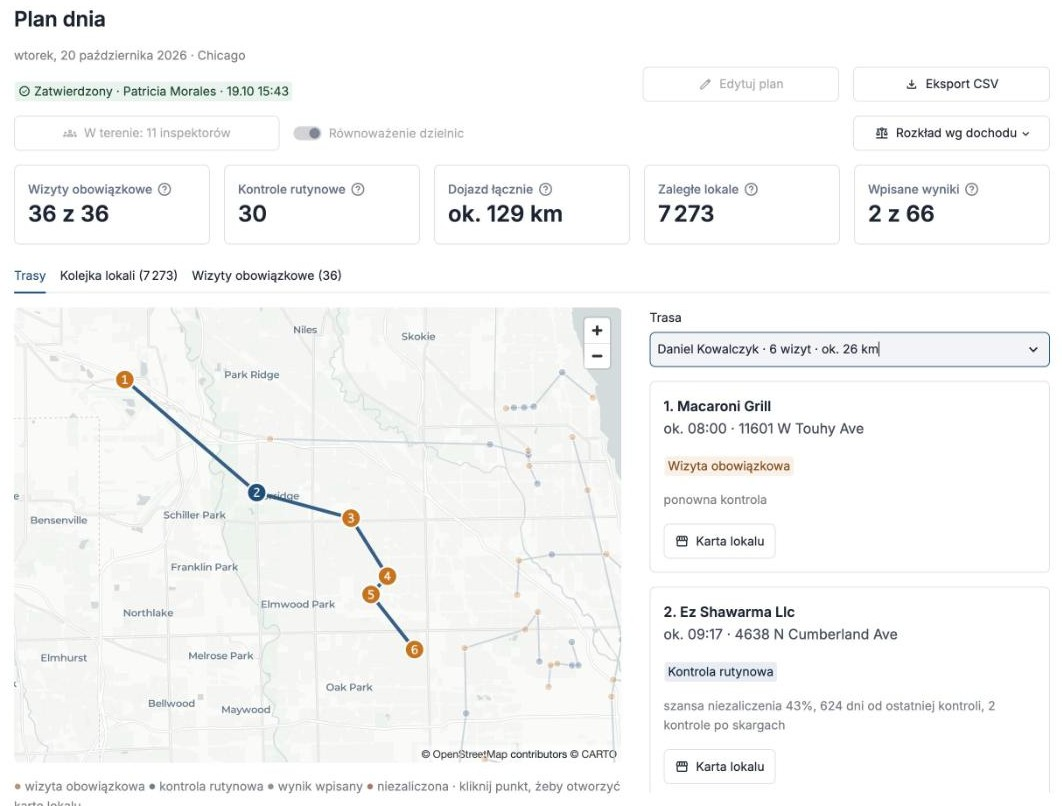
\includegraphics[width=0.72\textwidth, trim=0 190 0 0, clip]{../manager-plan.jpg}
\caption{Kierownik: plan dnia i trasa wybranego inspektora}
\end{subfigure}\\[0.6em]
\begin{subfigure}{\textwidth}\centering
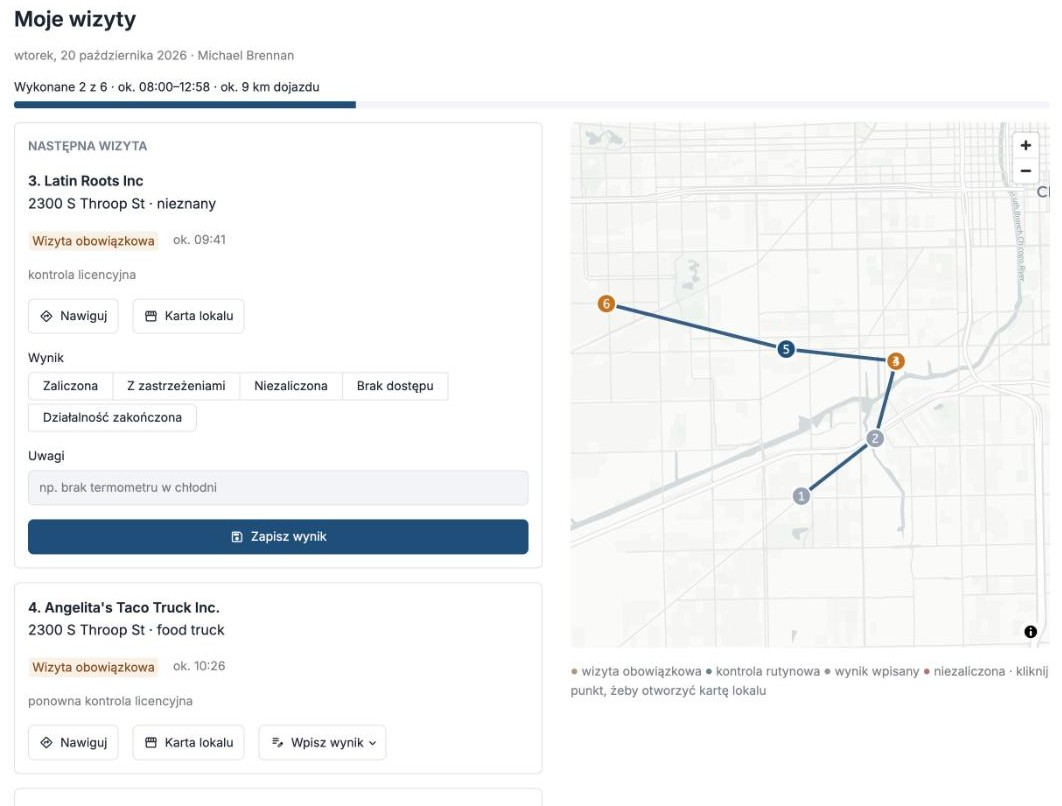
\includegraphics[width=0.72\textwidth, trim=0 290 0 0, clip]{../inspector-route.jpg}
\caption{Inspektor: następna wizyta, formularz wyniku i trasa}
\end{subfigure}
\caption{Prototyp. Kolor pomarańczowy oznacza zgłoszenia, granatowy kontrole rutynowe, szary
wizyty z wpisanym wynikiem; numery na mapie to kolejność wizyt.}
\label{fig:app}
\end{figure}

Osobna aplikacja (\texttt{report.py}) pokazuje wyniki oceny z rozdziałów~\ref{sec:eval}
i~\ref{sec:fair}; kod obu: \url{https://github.com/wojtke/chicago-inspections-dss}.

% =============================================================================================
\section{Ocena na danych historycznych}
\label{sec:eval}

System oceniono metodą, którą miasto zastosowało w 2014 roku do własnego
modelu~\cite{chicago2014}. Wybrano pięć okien po 60 dni z lat 2025--2026, których model
nie widział. W każdym oknie biorą udział kontrole rutynowe, które miasto faktycznie wykonało,
w lokalach znanych przed początkiem okna. Każda strategia ma dziennie tyle kontroli
rutynowych, ile wykonało miasto, i różni się tylko ich kolejnością. Wynik znany jest wyłącznie
dla kontroli, które się odbyły, dlatego nie można ocenić lokali, których miasto nie odwiedziło.

Mierzono średnie wyprzedzenie, czyli o ile dni wcześniej niż w kolejności faktycznej
odwiedzane są lokale z wynikiem negatywnym, osobno dla wszystkich lokali i dla placówek dla
dzieci i opieki zdrowotnej. Mierzono też odsetek tych lokali wykrytych w pierwszej połowie okna
oraz liczbę kilometrów na wizytę. Kilometry są miarą porównawczą, a nie rzeczywistym przebiegiem:
dla każdej strategii trasy liczy ten sam algorytm, tylko dla kontroli rutynowych.

\begin{table}[ht]
\centering\small
\caption{Strategie przy pełnym zespole, średnia z pięciu okien.}
\label{tab:policies}
\pgfplotstabletypeset[
  columns={name,days_sooner,high_impact_days_sooner,fails_first_half,km_per_visit},
  columns/name/.style={string type, column name={Strategia}, column type={@{}l}},
  columns/days_sooner/.style={column name={wszystkie}, fixed, fixed zerofill, precision=1, column type=c},
  columns/high_impact_days_sooner/.style={column name={dzieci i opieka}, fixed, fixed zerofill, precision=1, column type=c},
  columns/fails_first_half/.style={column name={wykryte w 1.~połowie}, fixed, precision=0, column type=c,
    postproc cell content/.append style={/pgfplots/table/@cell content/.add={}{\%}}},
  columns/km_per_visit/.style={column name={km na wizytę}, fixed, fixed zerofill, precision=1, column type={c@{}}},
  every head row/.style={before row={\toprule & \multicolumn{2}{c}{Wyprzedzenie (dni)} & & \\ \cmidrule(lr){2-3}},
                         after row=\midrule},
  every last row/.style={after row=\bottomrule},
]{data/policies.csv}
\end{table}

\begin{figure}[ht]
\centering
\begin{tikzpicture}
\begin{groupplot}[group style={group size=2 by 1, horizontal sep=1.7cm},
  width=0.47\textwidth, height=4.7cm]
  \nextgroupplot[xmin=0, xmax=59, ymin=0, ymax=100, xlabel={Dzień okna},
    ylabel={Wykryte lokale (\%)}, title={(a) wykrywanie w czasie}, title style={font=\small},
    legend to name=replaylegend, legend columns=4]
  \addplot[pol actual] table[x=day, y=actual]{data/curves.csv};   \addlegendentry{kolejność faktyczna}
  \addplot[pol random] table[x=day, y=random]{data/curves.csv};   \addlegendentry{losowa}
  \addplot[pol risk]   table[x=day, y=risk]{data/curves.csv};     \addlegendentry{tylko ryzyko}
  \addplot[pol system] table[x=day, y=system]{data/curves.csv};   \addlegendentry{pełny system}
  \nextgroupplot[x dir=reverse, xtick={70,80,90,100}, xticklabel={\pgfmathprintnumber{\tick}\%},
    xlabel={Wielkość zespołu}, ylabel={Wykryte w oknie (\%)}, ymin=25, ymax=100, title={(b) mniejszy zespół},
    title style={font=\small}]
  \addplot[pol actual, mark=o] table[x=team, y=actual_reached]{data/team.csv};
  \addplot[pol random, mark=none] table[x=team, y=random_reached]{data/team.csv};
  \addplot[pol risk, mark=square*, mark size=1.5pt] table[x=team, y=risk_reached]{data/team.csv};
  \addplot[pol system, mark=*, mark size=1.5pt] table[x=team, y=system_reached]{data/team.csv};
\end{groupplot}
\end{tikzpicture}\\[0.3em]
\pgfplotslegendfromname{replaylegend}
\caption{Odsetek lokali z wynikiem negatywnym wykrytych (a) do danego dnia okna przy pełnym
zespole i (b) w całym oknie przy mniejszym zespole. Średnia z pięciu okien. Linie kolejności
faktycznej i losowej niemal się pokrywają.}
\label{fig:replay}
\end{figure}

W pięciu badanych oknach kolejność faktyczna i losowa dały zbliżone średnie terminy wykrycia
(\DaysRandom{} dnia wyprzedzenia kolejności losowej). Sama
ocena ryzyka wykrywa lokale z wynikiem negatywnym najwcześniej, średnio o \DaysRisk{} dnia, ale
placówki dla dzieci i opieki zdrowotnej tylko o \DaysHiRisk{} dnia (tab.~\ref{tab:policies}).
Po uwzględnieniu wag AHP ogólne wyprzedzenie spada o \AhpLoss{} dnia, ale te placówki są
wykrywane o \DaysHiAhp{} dnia wcześniej. Wybór między tymi strategiami należy do kierownika
i wyrażają go wagi kryteriów. Trasy zmniejszają dojazd z \KmFair{} do \KmSys{} km na wizytę bez
utraty wyprzedzenia. Pełny system wyprzedza kolejność faktyczną średnio o \DaysSys{} dnia, a w
poszczególnych oknach od \SysDaysMin{} do \SysDaysMax{} dnia.

Rysunek~\ref{fig:replay}b pokazuje scenariusze mniejszego zespołu. Wizyty obowiązkowe zostają,
więc redukcja obejmuje tylko kontrole rutynowe: przy zespole mniejszym o 20\% zostaje ich
\CapEighty{} zamiast \CapFull{} w oknie, czyli \CapShareEighty\%. Kolejność faktyczna dociera
wtedy do \ReachCity\% lokali z wynikiem negatywnym, a pełny system do \ReachSys\%. Średnie
opóźnienie względem faktycznych terminów kontroli wynosi odpowiednio \LateCity{} i \LateSys{}
dnia. Lokale
nieodwiedzone liczone są tak, jakby odwiedzono je dzień po końcu okna, więc rzeczywiste
opóźnienie jest co najmniej takie.

% =============================================================================================
\section{Sprawiedliwość wobec dzielnic}
\label{sec:fair}

Sprawdzono, czy system nie traktuje gorzej dzielnic biedniejszych. Dla każdego kwintyla
dochodu liczony jest wskaźnik obciążenia: udział kwintyla we wczesnych wizytach (dla modelu:
we wskazaniach z górnych 10\%) podzielony przez jego udział w wynikach negatywnych. Wartość 1
oznacza wizyty proporcjonalne do rzeczywistych problemów, wartość wyższa nadmierne
kontrolowanie, niższa zbyt słabą ochronę.

\begin{figure}[ht]
\centering
\begin{tikzpicture}
\begin{groupplot}[group style={group size=2 by 1, horizontal sep=1.4cm},
  width=0.5\textwidth, height=4.1cm, ybar, ymin=0, ymax=2.05, xmajorgrids=false,
  xtick={1,...,5}, xticklabels={1\\najbiedniejsze, 2, 3, 4, 5\\najbogatsze}, xticklabel style={align=center},
  enlarge x limits=0.15, bar legend, legend style={at={(0.5,-0.35)}, anchor=north, legend columns=2}]
  \nextgroupplot[ylabel={Wskaźnik obciążenia}, bar width=7pt, title={(a) model, test 2025--2026},
    title style={font=\small}]
  \addplot[fill=light, draw=none] table[x=quintile, y=with_location]{data/burden_model.csv};
  \addlegendentry{ze współrzędnymi}
  \addplot[fill=navy, draw=none] table[x=quintile, y=without_location]{data/burden_model.csv};
  \addlegendentry{bez współrzędnych (używany)}
  \draw[ref line] (axis cs:0.4,1) -- (axis cs:5.6,1);
  \nextgroupplot[bar width=4.5pt, title={(b) plan, symulacja 2025--2026}, title style={font=\small}]
  \addplot[fill=city, draw=none] table[x=quintile, y=actual]{data/burden_plan.csv}; \addlegendentry{kolejność faktyczna}
  \addplot[fill=teal, draw=none] table[x=quintile, y=ahp]{data/burden_plan.csv}; \addlegendentry{ryzyko + AHP}
  \addplot[fill=plum, draw=none] table[x=quintile, y=ahp_fair]{data/burden_plan.csv}; \addlegendentry{AHP + równoważenie}
  \addplot[fill=navy, draw=none] table[x=quintile, y=system]{data/burden_plan.csv}; \addlegendentry{pełny system}
  \draw[ref line] (axis cs:0.4,1) -- (axis cs:5.6,1);
\end{groupplot}
\end{tikzpicture}
\caption{Wskaźnik obciążenia według kwintyla dochodu dzielnicy (1 = proporcjonalnie).}
\label{fig:fair}
\end{figure}

Współrzędne lokalu mogą pośrednio kodować zamożność dzielnicy. Model z nimi zyskuje tylko
\LocGain{} AUC na walidacji, a na teście wypada gorzej (\LocTestAuc{} wobec \AucTestGB).
Lokale z kwintyla \LocBurdenMaxQ{} wskazuje aż \LocBurdenMax{} raza częściej, niż wynikałoby
z ich udziału w wynikach negatywnych (rys.~\ref{fig:fair}a). Dlatego model nie korzysta ze
współrzędnych. Bez nich rozrzut maleje do \BurdenModelMin--\BurdenModelMax, choć kwintyl
\BurdenModelMaxQ{} nadal jest wskazywany częściej, niż wynikałoby z jego wyników. Model jest
podobnie skalibrowany w każdym kwintylu: średnie
przewidywanie różni się od faktycznego odsetka wyników negatywnych najwyżej o \CalGapMax{}
punktu procentowego. Wśród lokali wskazanych przez model (górne 10\%) od \FalseAlarmMin{} do
\FalseAlarmMax\% przechodzi kontrolę pozytywnie, we wszystkich kwintylach podobnie. AUC
w kwintylach wynosi od \AucQMin{} do \AucQMax.

W planie kolejność faktyczna daje wskaźnik obciążenia od \BurdenCityMin{} do \BurdenCityMax,
a samo AHP od \BurdenAhpMin{} do \BurdenAhpMax. Równoważenie zawęża ten przedział do
\BurdenFairMin--\BurdenFairMax{} (rys.~\ref{fig:fair}b). Trasowanie częściowo osłabia ten efekt
(\BurdenSysMin--\BurdenSysMax), bo grupuje wizyty geograficznie, więc rozrzut pełnego systemu
jest nieco większy niż kolejności faktycznej; najbiedniejszy kwintyl pozostaje na poziomie
\BurdenSysPoorest. W każdym kwintylu lokale z wynikiem negatywnym są wykrywane wcześniej niż
w kolejności faktycznej, od \QDaysSysMin{} do \QDaysSysMax{} dnia.

% =============================================================================================
\section{Ograniczenia}

\begin{itemize}
  \item Symulacja zmienia tylko kolejność kontroli, które się odbyły. Nie wiadomo, co inspektor
        znalazłby w lokalach, których miasto nie odwiedziło.
  \item Częstotliwość kontroli według kategorii ryzyka (182, 365 i 730 dni) jest założeniem,
        które trzeba sprawdzić w przepisach miasta.
  \item Czas wizyty, prędkość dojazdu i metryka miejska są przybliżeniami.
  \item Prototyp działa na danych historycznych: zgłoszenia danego dnia to kontrole obowiązkowe,
        które miasto wtedy wykonało. Zespół, plany i wyniki w wersji demonstracyjnej są fikcyjne.
        Model nie jest automatycznie trenowany na wynikach wpisanych w aplikacji.
  \item Dane o dochodzie dzielnic pochodzą z lat 2008--2012.
\end{itemize}

% =============================================================================================
\section{Podsumowanie}

Zbudowano system, który codziennie proponuje kierownikowi plan kontroli: najpierw wizyty
obowiązkowe, potem lokale o najwyższym priorytecie według wag AHP, rozdzielone na trasy
inspektorów. W symulacji na danych
z lat 2025--2026 przy tym samym zespole system wykrywa lokale z wynikiem negatywnym średnio
o \DaysSys{} dnia wcześniej niż kolejność faktyczna, a placówki dla dzieci i opieki zdrowotnej
o \DaysHiSys{} dnia wcześniej, przy mniejszym dojeździe. Model ma umiarkowaną trafność, dlatego
ostateczną decyzję podejmuje kierownik.

Podział pracy: Piotr odpowiadał za moduł predykcyjny (cechy, kalibracja), ocenę na danych
historycznych i audyt sprawiedliwości; Wojciech za moduł decyzyjny (AHP, ograniczenia, trasy),
architekturę i aplikację.

\begingroup\small\raggedright
\begin{thebibliography}{9}
\bibitem{foodinsp} City of Chicago, \textit{Food Inspections}, Chicago Data Portal,
  \url{https://data.cityofchicago.org/d/4ijn-s7e5}, dane do \DataUntil.
\bibitem{socio} City of Chicago, \textit{Community Areas}, \textit{Socioeconomic Indicators
  2008--2012}, Chicago Data Portal.
\bibitem{saaty} T.~L. Saaty, \textit{The Analytic Hierarchy Process}, McGraw-Hill, 1980.
\bibitem{platt} J.~Platt, \textit{Probabilistic Outputs for Support Vector Machines}, w: Advances in
  Large Margin Classifiers, MIT Press, 1999.
\bibitem{sklearn} F.~Pedregosa i in., \textit{Scikit-learn: Machine Learning in Python}, JMLR 12, 2011.
\bibitem{ortools} L.~Perron, V.~Furnon, \textit{OR-Tools}, Google,
  \url{https://developers.google.com/optimization}.
\bibitem{chicago2014} City of Chicago, \textit{Food Inspections Evaluation}, 2014,
  \url{https://github.com/Chicago/food-inspections-evaluation}.
\end{thebibliography}
\endgroup

\end{document}
